% tufte-handout.tex - DESC
% Iago Mosqueira - JRC. 2013
%
\documentclass{tufte-handout}

% ams
\usepackage{amssymb,amsmath}

% Set up the images/graphics package
\usepackage{graphicx}
\setkeys{Gin}{width=\linewidth,totalheight=\textheight,keepaspectratio}
\graphicspath{{graphics/}}

% natbib
\usepackage{natbib}
\bibliographystyle{plainnat}

% biblatex

% booktabs
\usepackage{booktabs}

% url
\usepackage{url}

% hyperref
\usepackage{hyperref}

% units.
\usepackage{units}

% fancyvrb
\usepackage{fancyvrb}
\fvset{fontsize=\normalsize}
\DefineShortVerb[commandchars=\\\{\}]{\|}
\DefineVerbatimEnvironment{Highlighting}{Verbatim}{commandchars=\\\{\}}


% multiplecol
\usepackage{multicol}

% lipsum
\usepackage{lipsum}

% These commands are used to pretty-print LaTeX commands
\newcommand{\doccmd}[1]{\texttt{\textbackslash#1}}% command name -- adds backslash automatically
\newcommand{\docopt}[1]{\ensuremath{\langle}\textrm{\textit{#1}}\ensuremath{\rangle}}% optional command argument
\newcommand{\docarg}[1]{\textrm{\textit{#1}}}% (required) command argument
\newenvironment{docspec}{\begin{quote}\noindent}{\end{quote}}% command specification environment
\newcommand{\docenv}[1]{\textsf{#1}}% environment name
\newcommand{\docpkg}[1]{\texttt{#1}}% package name
\newcommand{\doccls}[1]{\texttt{#1}}% document class name
\newcommand{\docclsopt}[1]{\texttt{#1}}% document class option name

% Shaded
\newenvironment{Shaded}{}{}
\newcommand{\KeywordTok}[1]{\textcolor[rgb]{0.00,0.44,0.13}{\textbf{{#1}}}}
\newcommand{\DataTypeTok}[1]{\textcolor[rgb]{0.56,0.13,0.00}{{#1}}}
\newcommand{\DecValTok}[1]{\textcolor[rgb]{0.25,0.63,0.44}{{#1}}}
\newcommand{\BaseNTok}[1]{\textcolor[rgb]{0.25,0.63,0.44}{{#1}}}
\newcommand{\FloatTok}[1]{\textcolor[rgb]{0.25,0.63,0.44}{{#1}}}
\newcommand{\CharTok}[1]{\textcolor[rgb]{0.25,0.44,0.63}{{#1}}}
\newcommand{\StringTok}[1]{\textcolor[rgb]{0.25,0.44,0.63}{{#1}}}
\newcommand{\CommentTok}[1]{\textcolor[rgb]{0.38,0.63,0.69}{\textit{{#1}}}}
\newcommand{\OtherTok}[1]{\textcolor[rgb]{0.00,0.44,0.13}{{#1}}}
\newcommand{\AlertTok}[1]{\textcolor[rgb]{1.00,0.00,0.00}{\textbf{{#1}}}}
\newcommand{\FunctionTok}[1]{\textcolor[rgb]{0.02,0.16,0.49}{{#1}}}
\newcommand{\RegionMarkerTok}[1]{{#1}}
\newcommand{\ErrorTok}[1]{\textcolor[rgb]{1.00,0.00,0.00}{\textbf{{#1}}}}
\newcommand{\NormalTok}[1]{{#1}}

\title{Tufte Handouts in rmarkdown}
\author{Michael Sachs}

\begin{document}
\maketitle

\section{Introduction}\label{introduction}

This is an R Markdown document. Markdown is a simple formatting syntax
for authoring HTML, PDF, and MS Word documents. \footnote{For more
  details on using R Markdown see \url{http://rmarkdown.rstudio.com}.}
This package provides output formats to create ``Tufte-style'' handouts.

Tufte-style handouts make heavy use of the right margin. Our package
provides templates for creating these types of documents in pdf or html
format. The pdf format uses the tufte-handout document class \footnote{Credit:
  \url{http://code.google.com/p/tufte-latex/}}. The html format uses
bootstrap with some css to put stuff in the margin. Each uses knitr
hooks to specify the types of figures.

\section{Usage}\label{usage}

To create sidenotes in html, some raw html is required. Place the
sidenote content between the tags
\texttt{\textless{}emph class="sidenote"\textgreater{}\textless{}/emph\textgreater{}}
to place them in the sidebar. In the pdf version, simply use the pandoc
footnote format \texttt{\^{}{[}Content{]}}.

The package provides two custom hooks for figure placement. The first is
\texttt{marginfigure}. Set \texttt{marginfigure = TRUE} in a chuck
option to place a figure in the right margin. Optionally, specify the
figure size and include a caption.

\begin{Shaded}
\begin{Highlighting}[]
\KeywordTok{library}\NormalTok{(ggplot2)}
\KeywordTok{ggplot}\NormalTok{(mtcars, }\KeywordTok{aes}\NormalTok{(}\DataTypeTok{y =} \NormalTok{mpg, }\DataTypeTok{x =} \NormalTok{wt)) +}\StringTok{ }\KeywordTok{geom_point}\NormalTok{() +}\StringTok{ }
\StringTok{    }\KeywordTok{stat_smooth}\NormalTok{(}\DataTypeTok{method =} \StringTok{"lm"}\NormalTok{)}
\end{Highlighting}
\end{Shaded}

\begin{marginfigure}
 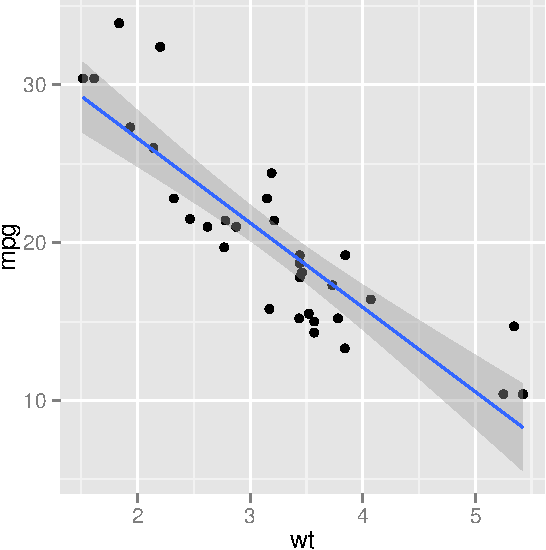
\includegraphics{./pindex_files/figure-latex/fig1}
\caption{ This is a marginfigure }
\end{marginfigure}

The second custom hook is \texttt{fig.star}. Setting
\texttt{fig.star = TRUE} creates a full-width figure spanning the main
body and the margin. Specify the width and height for best results.

\begin{Shaded}
\begin{Highlighting}[]
\KeywordTok{ggplot}\NormalTok{(faithful, }\KeywordTok{aes}\NormalTok{(}\DataTypeTok{y =} \NormalTok{eruptions, }\DataTypeTok{x =} \NormalTok{waiting)) +}\StringTok{ }
\StringTok{    }\KeywordTok{geom_point}\NormalTok{() +}\StringTok{ }\KeywordTok{stat_smooth}\NormalTok{(}\DataTypeTok{method =} \StringTok{"loess"}\NormalTok{)}
\end{Highlighting}
\end{Shaded}

\begin{figure*}
 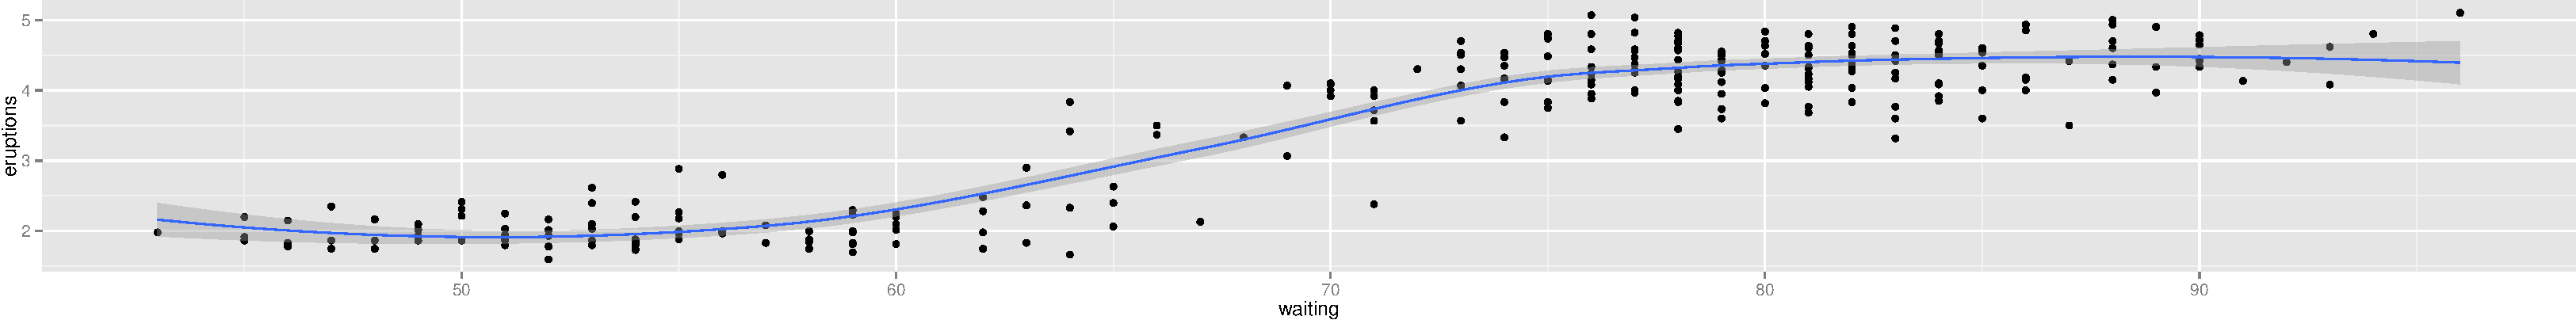
\includegraphics{./pindex_files/figure-latex/fig2}
\caption{ Full-width figure }
\end{figure*}

Finally, normal figures are plotted in the main body, with the captions
in the margin. The only option necessary here is the caption itself.

\begin{Shaded}
\begin{Highlighting}[]
\KeywordTok{ggplot}\NormalTok{(faithful, }\KeywordTok{aes}\NormalTok{(}\DataTypeTok{x =} \NormalTok{eruptions)) +}\StringTok{ }\KeywordTok{geom_histogram}\NormalTok{(}\DataTypeTok{binwidth =} \FloatTok{0.5}\NormalTok{)}
\end{Highlighting}
\end{Shaded}

\begin{figure}
 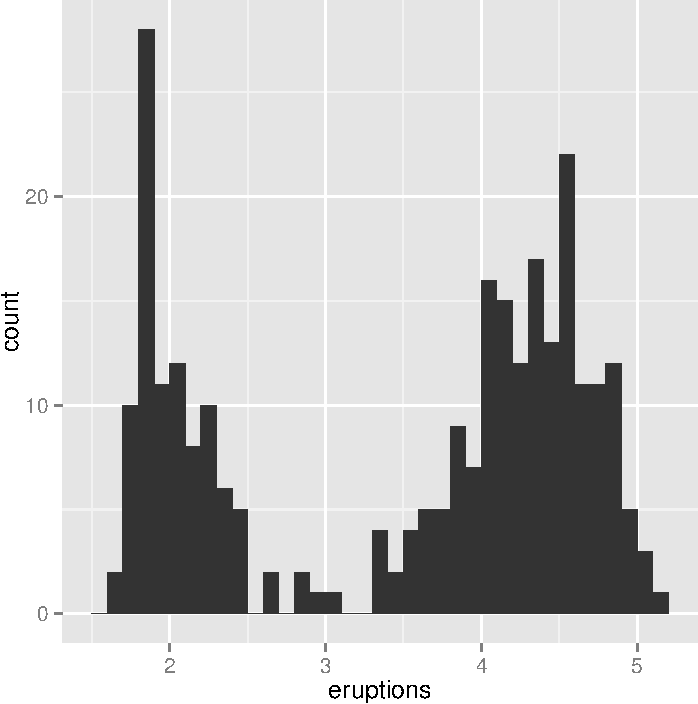
\includegraphics{./pindex_files/figure-latex/fig3}
\caption{ Normal figure with caption in the margin }
\end{figure}

\section{Resources}\label{resources}

Learn more about rmarkdown: \url{http://rmarkdown.rstudio.com}

\end{document}
